\section{Test design}

One of the benefits of having a microservice-based architecture is
the ability to scale different microservices independently, based on the
load on a particular service. Therefore, we designed our solution with that
goal in mind. Docker Compose allows scaling the number of replicas of
given containers (i.e. our microservices) via "docker-compose scale". To
perform scaling in an automated fashion we implemented an autoscaler through
a Python script. This script monitors the resource utilization per container
with a fixed cadence and decides whether to scale up, down or leave the single
microservices as they are. More specifically, the script gets resources information
using "docker stats" and, for every microservice, it increases or decreases the
number of replicas in the Docker compose depending on whether the usage is above
or below fixed thresholds.\\
In order to visualize and test the performances of the microservices under regular
and stress conditions, we utilized a series of tools. cAdvisor was used to extract
metrics from the containers, Prometheus to query cAdvisor and collect the necessary
metrics, and Grafana to show the metrics on charts and dashboards interactively
(Figure \ref{fig:grafana}).
The metrics are temporarily stored by these tools using Redis. Using this monitoring
system, it is easy to see the resources that are used by each container at any point in
time. To stress targeted containers, we decided to use the Pumba tool the leverages
the Linux stress-ng mechanism and sends workloads to Docker containers. It can be used
to stress a particular container for a given amount of time and this allows us to see
the metrics changing in the dashboard and the autoscaling mechanism operating on a
per-container basis.


\begin{figure}
    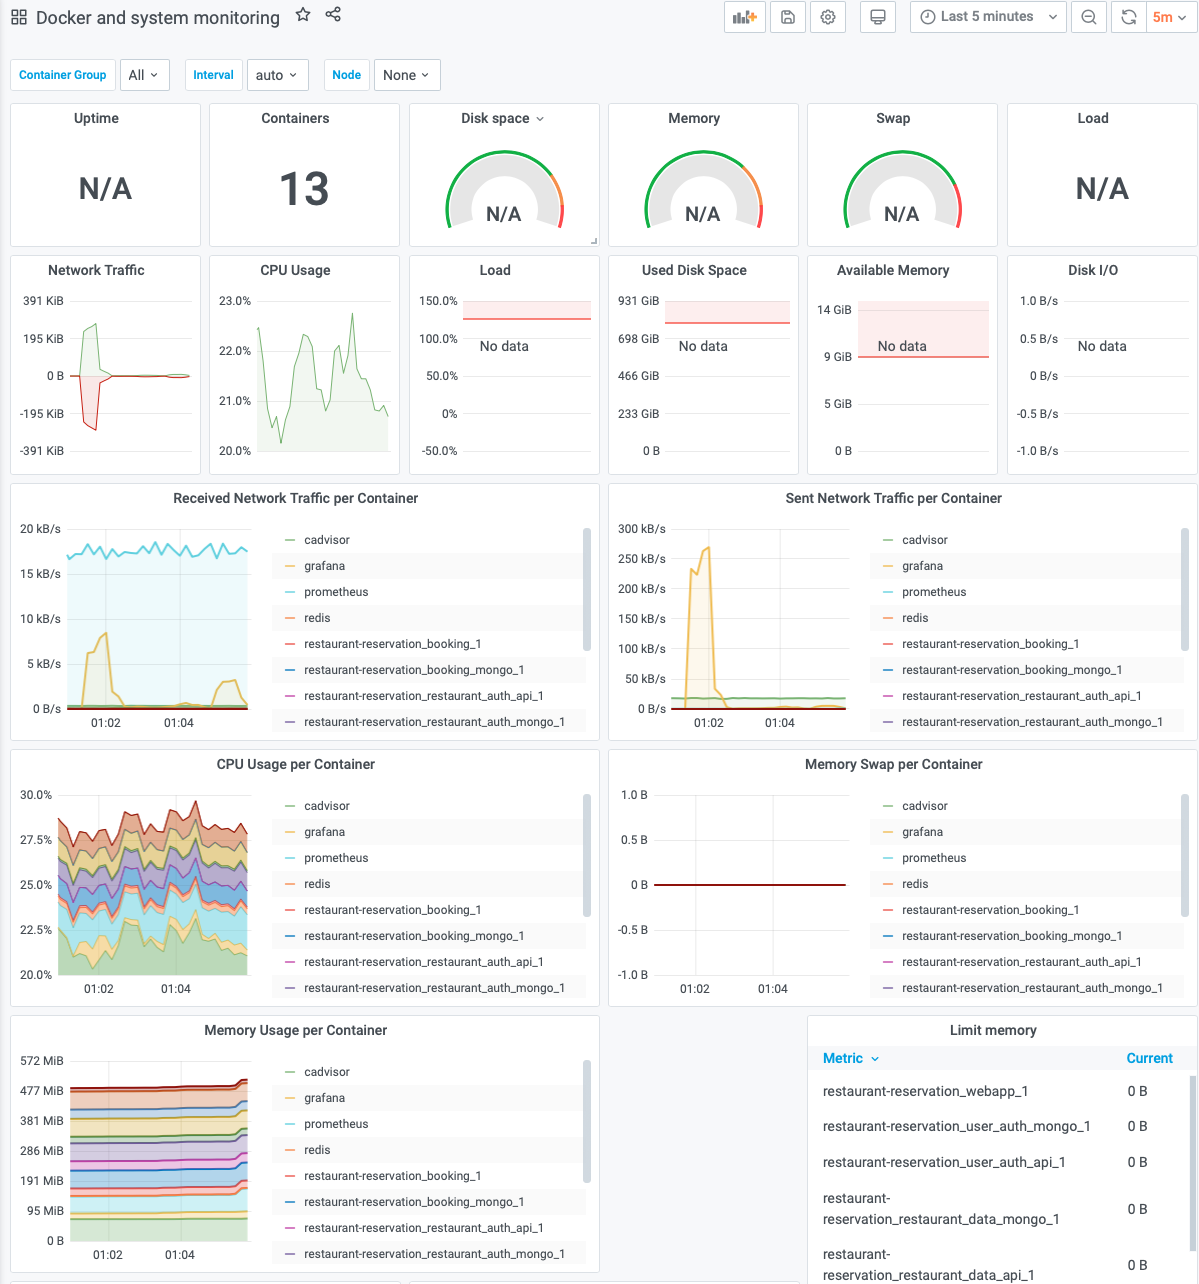
\includegraphics[width=\linewidth]{./images/grafana.png}
    \caption{Grafana metrics dashboard.}
    \label{fig:grafana}
\end{figure}